%%%%%%%%%%%%%%%%%%%%%%%%%%%%%%%%%%%%%%%%%%%%%%%%%%%%%%%%%%%%%%%%%%%%%%%%
%                                                                      %
%     File: Thesis_CNNsOnFPGAs.tex                                     %
%     Tex Master: Thesis.tex                                           %
%                                                                      %
%     Author: Pedro Miranda                                            %
%     Last modified :  26 Dec 2019                                     %
%                                                                      %
%%%%%%%%%%%%%%%%%%%%%%%%%%%%%%%%%%%%%%%%%%%%%%%%%%%%%%%%%%%%%%%%%%%%%%%%

\chapter{CNNs in Reconfigurable Hardware}
\label{chapter:CNNs_on_FPGAs}

CNNs have been implemented on multiple devices, from CPUs and GPUs to
FPGAs. CPUs and GPUs mostly use temporal architectures, while FPGAs, which are
in the class of reconfigurable hardware devices use spatial architectures to
achieve parallelization. Another type of reconfigurable hardware devices is the
Coarse Grained Reconfigurable Array (CGRA) architecture, which, despite
powerful, is not as studied as FPGAs for the implementation of CNNs, and is the
main focus of this work.

An effective parallelization is specially important in the convolutional layers
which are responsible for $90\%$ of the execution time during inference
\cite{hal:accelCNNonFPGA}.

This chapter focusses on the main techniques used to accelerate convolutional
layers in Reconfigurable Hardware. First, the inherent parallelisms of the
convolutional algorithm are highlighted, followed by a presentation of the main
optimization techniques used. Closing the chapter, the Deep Versat CGRA, which
will be used in this work, is reviewed.

\section{General CNN Algorithm}
\label{sec:data_and_general_CNN_algorithm}
The data used in a convolution is presented in
Fig.~\ref{fig:data_representation}. A particular layer has an input $X$ composed
of $C$ FMs of size ($W\times H$) and uses $N$ kernels ($\Theta_1$ to $\Theta_N$)
of size ($J\times K \times C$) to obtain the output $Y$ composed of $N$ FMs of
size ($V\times U$). The generic CNN algorithm is presented in
Alg.~\ref{alg:general_CNN}. The bias is not represented for simplicity.
%The output $Y$ of a particular layer is obtained using the input $X$ and the
%kernels $\Theta_1$ to $\Theta_N$ in the generic CNN algorithm presented in
%Alg.~\ref{alg:general_CNN}. The bias is not represented for simplicity.

\begin{figure}[!htb]
	\centering
	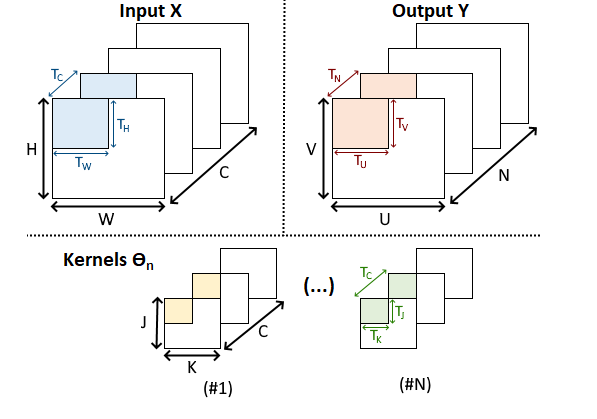
\includegraphics[width=0.5\textwidth]{Figures/data_representation.png}
	\caption[Caption for figure in TOC.]{Input pixels, kernels and output pixels representation, adapted from \cite{hal:accelCNNonFPGA}}
	\label{fig:data_representation}
\end{figure}

\begin{algorithm}
	\caption{General CNN algorithm for a single layer.}
	\label{alg:general_CNN}
	\begin{algorithmic}
		\FOR[\ // Loop 4 iterates over the $N$ channels of output $Y$]{$n \in \{1, \dots, N\}$} 
		\FOR{$v \in \{1,\dots,V\}$}
		\FOR[\ // Loop 3 iterates over the pixels within the same output FM]{$u \in \{1,\dots,U\}$} 
		\FOR[\ // Loop 2 iterates over the channels of input $X$]{$c \in \{1,\dots,C\}$} 
		\FOR{$k \in \{1,\dots,K\}$}
		\FOR[\ // Loop 1 iterates over a 2D kernel window]{$j \in \{1,\dots,J\}$}
		\STATE MACC: $Y[u, v, n] += X[j, k, c] \times \Theta_n [j, k] $
		\ENDFOR
		\ENDFOR
		\ENDFOR
		\ENDFOR
		\ENDFOR
		\ENDFOR	
	\end{algorithmic}
\end{algorithm}

The commented loops are candidates for loop unrolling, as discussed in section~\ref{sec:loop_unrolling}.
%Alg.~\ref{alg:general_CNN} has four different types of loops.
%\begin{itemize}
%	\item Loop 4 iterates over the $N$ channels of output $Y$.
%	\item Loop 3 iterates over the pixels within the same output FM.
%	\item Loop 2 iterates over the channels of input $X$.
%	\item Loop 1 iterates over a 2D kernel window.
%\end{itemize}


%The algorithm has four different parallelization opportunities, one for each of the commented loops in Alg.~\ref{alg:general_CNN}.
%\begin{itemize}
%	\item Loop 4 exhibits \underline{Inter-FM parallelism}, meaning that each output FM can be calculated in parallel. For each output FM the same input pixels are used, but a different kernel $\Theta_n$ is required.
%	\item Loop 3 presents \underline{Intra-FM parallelism} by calculating multiple output pixels within the same FM. This process uses the same kernel $\Theta_n$, but different input pixels.
%	\item Loop 2 highlights \underline{Inter-convolution parallelism} as each 3D convolution can be described as a sum of multiple 2D convolutions across the input FMs. Each 2D convolution requires different data from the input and kernel.
%	\item Loop 1 reveals \underline{Intra-convolution parallelism} as each 2D convolution at the two innermost loops can be implemented concurrently. As happens for Loop 2, there is no common data used at each Loop 1 iteration.
%\end{itemize}

 %Loop 4 exhibits \underline{Inter-FM parallelism}, meaning that each output FM can be calculated in parallel. For each output FM the same pixels are used, but a different kernel $\Theta_n$ is required. Loop 3 presents \underline{Intra-FM parallelism} by calculating multiple output pixels within the same FM. This process uses the same kernel $\Theta_n$, but different input pixels. Loop 2 highlights \underline{Inter-convolution parallelism} as each 3D convolution can be described as a sum of multiple 2D convolutions across the input FMs. Each 2D convolution requires different data from the input and kernel. Loop 1 reveals \underline{Intra-convolution parallelism} as each 2D convolution at the two innermost loops can be implemented concurrently. As happens for Loop 2, there is no common data used at each Loop 1 iteration.

\section{CNN Inference Acceleration in FPGAs}
\label{sec:CNN_inference_acceleration}
In general, acceleration for CNN inference in FPGA is done by a combination of \underline{datapath} and \underline{CNN model} optimizations.
%The algorithmic optimizations consist in transforming the convolution into either a general matrix multiplication (GEMM) or resorting to a Winograd transformation or Fast Fourier Transform (FFT).

Datapath optimizations explore parallelism opportunities in the convolutional algorithm described in~\ref{sec:data_and_general_CNN_algorithm}. However due to resource limitations in the devices when compared with the amount of calculations done in a single convolutional layer, only some parallelisms can be explored.

The last optimization type consists in trading model accuracy to improve computational and energy efficiency. This can be achieved by operating over reduced precision operands or reducing the model size.

% FPGA acceleration techniques:
%	Algorithmic
%	Datapah Optimization
%	CNN Model optimization
%	HW Generation (dont talk about this)
% describe what I will use: Datapath and Quantization (Fixed Point)

%\section{Algorithmic Optimizations}
%\label{sec:Algorithmic_Opt}
%The GEMM is commonly used in CPUs and GPUs, having large memory requirements to replicate the kernels into matrix form. Implementations in FPGA avoid replicating the kernels by generating the access pattern of the convolution.
%
%The FFT transform is interesting for convolutions with kernels with size over ($5 \times 5$) \cite{hal:accelCNNonFPGA}, which are increasingly less common as networks for image processing tend to have $3 \times 3$ kernels.
%
%The Winograd transform presents particular efficiency for kernels with size equal or smaller than ($3 \times 3$), by reducing the amount of multiplications done in exchange for more additions. In FPGAs, the multiplications and additions have the same computational cost if the MACs are done exclusively in DSP blocks. In fact, with the Winograd transform, the total number of operations increases, making it less efficient than the regular convolution algorithm.% Furthermore, this method requires complex processing of the weights before inference deployment.\\

\section{Datapath Optimizations}
\label{sec:Datapath_Optimizations}
%The resource limitations of FPGA devices when contrasted with current CNNs, make the complete exploitation of all parallelisms referenced in \ref{sec:data_and_general_CNN_algorithm} impossible. 
In~\cite{hal:accelCNNonFPGA}, SIMD accelerators are presented as the main strategy for implementing datapath optimizations. The architecture of a generic SIMD accelerator is presented in Fig.~\ref{fig:SIMD_accel}. SIMD accelerators receive the input FMs and weights from external memory into an on-chip buffer. This data is then processed in a pool of PEs that output the results into an output buffer. The output is then sent back to the external memory. Each PE contains on-chip registers and performs the computations using DSP blocks.
%this paragraph comes from the (3.5) Memory Accesses in CNNs section, now commented
The two levels of caching implemented by the on-chip buffers and registers reduce the accesses to external memory. This reduction has a significant impact in terms of power consumption, since the accesses to external memory are the determinant factor for power consumption in FPGAs~\cite{sze:dnn_tutorial, hal:accelCNNonFPGA}.

%The main strategies used resort to SIMD accelerators. SIMD accelerators, Fig.~\ref{fig:SIMD_accel}, receive the input FMs and weights from external memory into a buffer. This data is then send to a pool of PEs that output the results into an output buffer. The output is then sent back to the external memory. Each PE contains on-chip registers and perform the computations using DSP blocks.

%The datapath optimization consists in finding the architectural configuration
%that maximizes the computational throughput.
With this accelerator architecture, the process of datapath optimization consists in finding the configuration of the PEs and data schedule that maximizes computational throughput, specially for convolutions.

Since the convolution is a set of nested loops (Alg.~\ref{alg:general_CNN}),
loop optimization techniques as \underline{loop unrolling}, \underline{loop
  tiling} and \underline{loop interchange} are applied.


\begin{figure}[!htb]
	\centering
	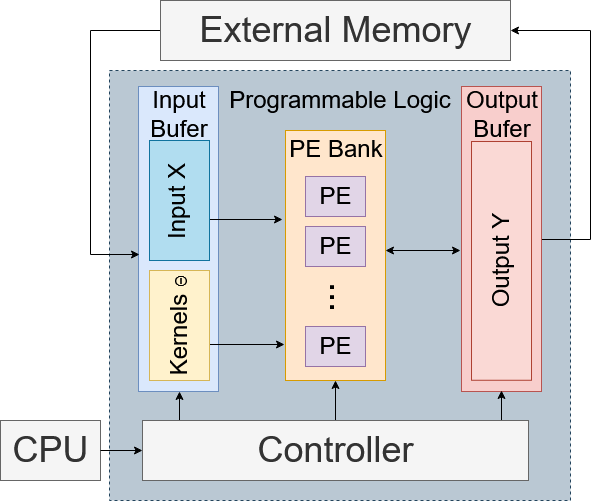
\includegraphics[width=0.5\textwidth]{Figures/SIMDAccelerator.png}
	\caption[Caption for figure in TOC.]{SIMD Accelerator, adapted from~\cite{hal:accelCNNonFPGA}}
	\label{fig:SIMD_accel}
\end{figure}

\subsection{Loop Unrolling}
\label{sec:loop_unrolling}
%In Alg.~\ref{alg:general_CNN} there are four highlighted loops that lead to
%different dataflows.
In Alg.~\ref{alg:general_CNN}, there are four parallelization opportunities, one for each of the commented loops, each one leading to a different dataflow.


\begin{itemize}
	\item Loop 4, which iterates over the output channels, exhibits \underline{Inter-FM parallelism}, meaning that each output FM can be calculated in parallel. For each output FM the same input pixels are used, but a different kernel $\Theta_n$ is required. By unrolling loop 4, at each cycle, the same pixel is multiplied by a corresponding
	weight from different kernels. This leads to an uniform access for input pixels
	and kernels. All computed values belong to pixels in different output FMs, so
	all of them need to be stored for the next cycle.
	\item Loop 3, which iterates over the pixels within the same output FM, presents \underline{Intra-FM parallelism} by calculating multiple output pixels within the same FM. This process uses the same kernel $\Theta_n$, but different input pixels. Unrolling Loop 3 requires accessing different pixels within the same FM, but
	enables the reuse of the weights. All the computed values belong to a different
	output pixel, so the number of partial values that need to be stored corresponds
	to the unroll factor applied to this loop.
	\item Loop 2, which iterates over the input channels, highlights \underline{Inter-convolution parallelism} as each 3D convolution can be described as a sum of multiple 2D convolutions across the input FMs. Each 2D convolution requires different data from the input and kernel. Unrolling Loop 2 leads to an uniform access for input pixels and weights in input FM and 2D kernel coordinates. However each value pair comes from a different
	channel. All the calculated values can be added into a single partial sum.
	\item Loop 1, which iterates over a 2D kernel window, reveals \underline{Intra-convolution parallelism} as each 2D convolution at the two innermost loops can be implemented concurrently. As happens for Loop 2, there is no common data used at each Loop 1 iteration. Unrolling Loop 1 requires accessing different input and weight positions at the
	same channel. This requires a complex address generation. All the calculated
	values are used for the same output pixel, therefore can be added, requiring the
	storage of only one partial sum value.
\end{itemize}
%Unrolling Loop 1 requires accessing different input and weight positions at the
%same channel. This requires a complex address generation. All the calculated
%values are used for the same output pixel, therefore can be added, requiring the
%storage of only one partial sum value.
%
%Unrolling Loop 2 leads to an uniform access for input pixels and weights in (x,
%y) and (j, k) coordinates. However each value pair comes from a different
%channel. All the calculated values can be added into a single partial sum.
%
%Unrolling Loop 3 requires accessing different pixels within the same FM, but
%enables the reuse of the weights. All the computed values belong to a different
%output pixel, so the number of partial values that need to be stored corresponds
%to the unroll factor applied to this loop.
%
%For loop 4, at each cycle, the same pixel is multiplied by a corresponding
%weight from different kernels. This leads to an uniform access for input pixels
%and kernels. All computed values belong to pixels in different output FMs, so
%all of them need to be stored for the next cycle.
%
%The chosen method of loop unrolling influences the parallelism scheme used and
%the number of multipliers required.

\subsection{Loop Tiling}
\label{sec:loop_tiling}
Loop tiling is used if the input data in deep CNNs is too large to fit in the on-chip
memory at the same time~\cite{hal:accelCNNonFPGA}. Loop tiling divides the data into blocks, like in
Fig.~\ref{fig:data_representation}, that are placed in the on-chip memory. The
main goal of this technique is to assign the tile size in a way that leverages
the data locality of the convolution and minimizes the data transfers from and
to external memory. Ideally, each input and weight is only transferred once from
external memory to the on-chip buffers.

If the kernel size is bigger than the stride ($J>Stride\text{ or }K>Stride$),
the resulting tiles overlap each other at the boundaries. The added amount of
reads is negligible when compared with the tile area~\cite{Ma:80_OptDataflow_in_CNN}.

The tiling factors set the lower bound for the size of the on-chip buffer.

\subsection{Loop Interchange}
\label{sec:loop_interchange}
Loop interchange sets the execution order of the four loops. The innermost loop
is the first to be computed and the outermost loop is the last to be completed.

The loop interchange can be divided into intra-tiling and inter-tiling loop
order. The intra-tiling loop order determines the dataflow from the on-chip
memory to the PEs, since the data belongs to the same tile loaded into the
on-chip buffer. While the inter-tiling loop order sets the dataflow from
external memory to the on-chip memory, by defining the order of the tiles loaded
into the on-chip buffer.

\subsection{Design Space Analysis}
\label{sec:datapath_opt_analysis}
In~\cite{Ma:80_OptDataflow_in_CNN}, the loop optimization techniques presented in sections~\ref{sec:loop_unrolling} to~\ref{sec:loop_interchange} are used to perform an analysis of the SIMD accelerators design space.


The development of the accelerator in~\cite{Ma:80_OptDataflow_in_CNN} is guided by the minimization of the
\underline{computing latency}, the requirements of \underline{partial sum
  storage} and the accesses to the \underline{external memory} and
\underline{on-chip buffer}.

The computing latency has a lower bound determined by the number of multipliers
available. However, if the ratios between the loop tiling factors and unroll
factors are not integers, the amount of multiplications done in parallel are less than the number of available multipliers. 
%FIX; what is underutilized in this case ???? bandwidth?
The same
happens if the ratio between the total data size and the tile size is not
integer with regards to the external memory transactions. 
% END FIX (FIXED)
To avoid the
underutilization of the resources, the chosen loop tiling factors should be
common factors of the total data size, the same needs to happen between the loop
tiling and unrolling factors.

The amount of partial sums that need to be stored depends mainly on the order of
loop computations. To reduce the number of stored partial sums the output pixel
values need to be computed as early as possible. This corresponds to having Loop
1 as the innermost loop.

The accesses to the external memory are tied to the size of the on-chip buffers,
which in turn have a size lower bound determined by the loop tiling factors.

The accesses to the on-chip buffers can be reduced by reusing the data sent to
the PEs. According to the analysis in~\ref{sec:loop_unrolling}, this corresponds
to unrolling Loop 3 and Loop 4.

\subsection{FPGA Implementation}
\label{sec:proposed_accelerator}
In~\cite{Ma:80_OptDataflow_in_CNN}, an accelerator architecture is implemented based on the impact of the loop optimizations in performance.

The accelerator proposed in~\cite{Ma:80_OptDataflow_in_CNN} unrolls loops 3 and 4, which minimizes the
on-chip memory accesses.

The tilling is done across W and H of the input data and V and N of the output
data. This tiling choice guarantees that the data for Loop 1 and Loop 2 is
always buffered and can be computed in sequence. In turn, this reduces the
amount of saved partial sums to the product of the unrolling
factors. Furthermore, the row tiling at the output requires sequential memory
accesses which benefit from DMA data transfers.

Tab.~\ref{tab:Ma_comparison} presents a comparison between the works
in~\cite{Ma_comp_ref10, Ma_comp_ref9, Ma_comp_ref8, Ma:80_OptDataflow_in_CNN},
which implement the VGG~\cite{VGG} network in FPGA.

The proposed accelerator in~\cite{Ma:80_OptDataflow_in_CNN} achieves over three
times the throughput of the other accelerators. The results highlight the impact in
computational throughtput of the datapath optimization strategies. For example, between implementations~\cite{Ma_comp_ref8} and~\cite{Ma:80_OptDataflow_in_CNN}, 
the same network, at the same frequency achieves over three times the throughput.
%The main difference between the
%accelerators is the datapath optimization strategy.

%Although the exact number of used DSP blocks and on-chip memory is not known
%for two of the implementations, the

\begin{table}[!htb]
	\renewcommand{\arraystretch}{1.2} % more space between rows
	\centering
	\caption[Table caption shown in TOC.]{Comparison of CNN FPGA implementations, adapted from~\cite{Ma:80_OptDataflow_in_CNN}}
	\label{tab:Ma_comparison}
	\begin{threeparttable}
	\begin{tabular}{|c|c|c|c|c|}
		\hline
		Network [Implementation]     & VGG~\cite{Ma_comp_ref10}	& VGG~\cite{Ma_comp_ref9} & VGG~\cite{Ma_comp_ref8} & VGG~\cite{Ma:80_OptDataflow_in_CNN}  \\ \hline
		FPGA      			 & Zynq XC7Z045 & Stratix-V GSD8 & Virtex-7 VX690t & Arria-10 GX 1150    \\  \hline
		Frequency (MHz)		& 150			& 120			&150				&	150			\\  \hline
		%\# Operations (GOP)  	 & 	30.76		&	30.95		&	30.95			&30.95				\\   \hline
		Number of Weights	& 50.18 M		&	138.3 M		&138.3 M			&138.3 M				\\  \hline
		%Precision (all fixed) & 16 bit		&	8 - 16 bit	&	16 bit			&8 - 16 bit				\\  \hline
		DSP Utilization 	& 780 (89\%)	& 1,963\tnote{b}		&	3,600\tnote{b}			&1,518 (100\%)				\\  \hline
		%Logic Utilization  & 				&				&					&				\\  \hline
		On-chip RAM\tnote{a}			& 486 (87\%)	& 2,567\tnote{b}		&1,470\tnote{b}				&1,900 (70\%)				\\  \hline 
		Latency/Image (ms) & 224.6			&262.9			&151.8				&47.97				\\  \hline
		Throughput (GOPS)	&136.97			&117.8			&203.9				&645.25				\\ \hline
		Unrolled Loops		& 1,2,4		& 1,2,4				& 1,2,4					& 3,4				\\ \hline
	\end{tabular}
		\begin{tablenotes}
	\item[a] Xilinx FPGAs in BRAMs (36 Kb) and Altera FPGAs in M20K RAMs (20 Kb)\\
	\item[b] The resource utilization is not reported in the original papers. The total available resources of the used FPGAs are listed
\end{tablenotes}
\end{threeparttable}
\end{table}


%\begin{table}[!htb]
%	\renewcommand{\arraystretch}{1.2} % more space between rows
%	\centering
%	\caption[Table caption shown in TOC.]{Comparison of CNN FPGA implementations, adapted from \cite{Ma:80_OptDataflow_in_CNN}}
%	\label{tab:Ma_comparison}
%	\begin{threeparttable}
%	\begin{tabular}{|c|c|c|c|}
%		\hline
%		Network           	& VGG 			& VGG			  & VGG  \\ \hline
%		FPGA      			 & Zynq XC7Z045 & Stratix-V GSD8  & Arria-10 GX 1150    \\  \hline
%		Frequency (MHz)		& 150			& 120				&	150			\\  \hline
%		%\# Operations (GOP)  	 & 	30.76		&	30.95				&30.95				\\   \hline
%		Number of Weights	& 50.18 M		&	138.3 M			&138.3 M				\\  \hline
%		%Precision (all fixed) & 16 bit		&	8 - 16 bit			&8 - 16 bit				\\  \hline
%		DSP Utilization 	& 780 (89\%)	& 1,963\tnote{b}		&1,518 (100\%)				\\  \hline
%		On-chip RAM\tnote{a}			& 486 (87\%)	& 2,567\tnote{b}		&1,900 (70\%)				\\  \hline 
%		Latency/Image (ms) & 224.6			&262.9			&47.97				\\  \hline
%		Throughput (GOPS)	&136.97			&117.8			&645.25				\\ \hline
%		Unrolled Loops		& 1,2,4		& 1,2,4		& 3,4				\\ \hline
%	\end{tabular}
%		\begin{tablenotes}
%			\item[a] Xilinx FPGAs in BRAMs (36 Kb) and Altera FPGAs in M20K RAMs (20 Kb)\\
%			\item[b] The resource utilization is not reported in the original papers. The total available resources of the used FPGAs are listed
%		\end{tablenotes}
%	\end{threeparttable}
%\end{table}


%\section{Mapping of Other Layers}
%\label{sec:mapping_other_layers}

\section{CNN Model Optimization}
\label{sec:CNN_model_opt}

The two most common methods for CNN model optimization in FPGA
devices are \underline{operand quantization}  and \underline{operation reduction}.
These methods reduce the amount of resources required, enabling more
parallelization and reducing the data transfers.

CNN model optimizations need to take into account the accuracy loss of the
model. In order to minimize the accuracy loss, these methods are integrated into
the model training phase.

%The CNN model optimization is implemented in FPGA devices by two main methods:
%\underline{operand quantization} or \underline{operation reduction}. These
%methods reduce the amount of resources required, which enables more
%parallelization and reduce the data transfers, which is the main factor for
%energy consumption.
%
%The performed approximations need to take in account the accuracy loss of the
%model. For further accuracy loss minimization, these methods are integrated into
%the training phase of the model.

\subsection{Quantization}
\label{sec:quantization}
Quantization is done by reducing the operand bit size. This restricts the
operand resolution, affecting the resolution of the computation
result. Furthermore, representing the operands in fixed-point instead of
floating-point translates into another reduction in terms of required resources
for computation.
% For example, a DSP block can perform two $18\times 19$ independent fixed point multiplications, while only being able to do one floating point multiplication.\\

The simplest quantization method consists in setting all weights and inputs to
the same format across all layers of the network. This is referred as static
fixed point (SFP). However, the intermediate values still need to be bit-wider
to prevent further accuracy loss.

In deep networks, there is a significant variation of data ranges across the
layers. The inputs tend to have larger values at latter layers, while the
weights for the same layers are smaller in comparison. The wide range of values
makes the SFP approach inviable, since the bit-width needs to expand to
accommodate all values.

This problem is addressed by Dynamic Fixed Point (DFP), which consists in the
attribution of different scaling factors to the inputs, weights and outputs of
each layer.

%The most common quantizations involve a linear mapping with uniform distance
%between each quantization level. Other common approaches use a simple mapping
%function like the log function that can be easily implemented in hardware.
%FIX este paragrafo é impossivel de perceber. Qual a relação entre distance e scale factor? Desde quando o log é facil de implementar em hw se ha teses de doutoramento sobre o assunto? (FIXED) - mais vale nem falar disto

In~\cite{Ma:ALAMO}, a DFP implementation with 8 bits for the weights and 10 bits
for the pixel values, without fine-tuning of the weights, is presented. The DFP
implementations yielded minimal accuracy losses for the networks tested, as is
presented in Tab.~\ref{tab:quantization_from_ALAMO}. The fixed-point precision
representation leads to an accuracy loss of less than 1\%.

\begin{table}[!htb]
	\renewcommand{\arraystretch}{1.2} % more space between rows
	\centering
	\begin{tabular}{|c|c|c|c|c|}
		\hline
		\textbf{\begin{tabular}[c]{@{}c@{}}Model Accuracy\\ Comparison\end{tabular}} & \multicolumn{2}{c|}{\textbf{\begin{tabular}[c]{@{}c@{}}Full \\ Precision\end{tabular}}} & \multicolumn{2}{c|}{\textbf{\begin{tabular}[c]{@{}c@{}}Fixed-Point \\ Precision\end{tabular}}} \\ \hline
		\textbf{CNN Model}                                                           & \textbf{Top-1}                             & \textbf{Top-5}                             & \textbf{Top-1}                                 & \textbf{Top-5}                                \\ \hline
		AlexNet~\cite{AlexNetKrizhevsky:2012}                                                                      & 56.78\%                                    & 79.72\%                                    & 55.64\%                                        & 79.32\%                                       \\ \hline
		NIN~\cite{NIN:cnnModel}                                                                          & 56.14\%                                    & 79.32\%                                    & 55.74\%                                        & 78.96\%                                       \\ \hline
	\end{tabular}
	\caption[Table caption shown in TOC.]{Accuracy Comparison with the ImageNet dataset, adapted from~\cite{Ma:ALAMO}}
	\label{tab:quantization_from_ALAMO}
\end{table}

\subsection{CNN Model Reduction}
\label{sec:CNN_prunning}
Another way to optimize the CNN model is to reduce the amount of computations
necessary for inference. One method to achieve this is through
\underline{weight pruning}. %Unlike
%quantization, CNN model reduction requires retraining of the weights.

Weight pruning consists in eliminating or zeroing the lowest weights. After
that, the remaining weights are fine-tuned in order to improve the
accuracy. Other criteria for pruning can be developed, like energy based
approaches. In~\cite{Yang_Energy-prunning} the energy consumption of each layers is estimated
by accounting for the accesses to the multiple memory levels and the energy expended for computation.
The amount of energy estimated by a layer determines the order in which the layers are pruned.
The more energy demanding layers are pruned first, since the first layers being pruned tend
to have better compression ratios than following layers.
%FIX se referes energy-based explica! (FIXED)

%The low rank approximation reduces the computation by replacing the convolution
%of a 3D kernel by three successive 1D filters. This
%is possible if the kernel has low rank to begin with, meaning that all the columns 
%in a 2D kernel are linearly dependent. The same for 
%With this alteration a 3D
%convolution requires $J+K+C$ multiplications instead of $J\times K\times C$. To obtain low rank
%kernels, the cost function during training can be altered to promote kernels
%with such characteristics. Another option is to approximate a kernel by a
%succession of low rank filters, resulting in $r\times (J+K+C)$ multiplications.
% FIX: o que é low rank? o que é J, K, C? (não vou virar a pagina para ver) Porque dá um resultado aproximado com muitas menos mults?
% paragrafo totalmente inaceitável : ou explicas ou apagas (FIXED) - isto até é muito interessante, mas levava a uma explicação alongada que também não é o foco do trabalho

Tab.~\ref{tab:model_reduction_comp} presents results achieved by CNN model
reduction techniques. Both implementations manage to remove the majority of the
weights without significant impact in accuracy. In
fact,~\cite{Hal_model_reduction_ref45,
  Hal_model_reduction_ref7} claim an accuracy reduction within 1\% when compared
with the respective model using all parameters.
% FIX all implementations como se a primeira é Low rank? Ou será low Rank + Prunning? São todas os só as Pruning? 
%(FIXED) - como não falo de SVD/low rank também não incluo na tabela


\begin{table}[]
	\centering
	\begin{tabular}{|l|c|c|c|c|}
		\hline
		\multicolumn{1}{|c|}{\textbf{Optimization}} & \textbf{Dataset}  & \textbf{Removed Parameters (\%)} & \textbf{Accuracy (\%)} & \textbf{Bitwidth}       \\ \hline
%		Low rank~\cite{Hal_model_reduction_ref9}                           & ImageNet & 63.6                    & 87.96         & 16 Fixed Point \\ \hline
		Prunning~\cite{Hal_model_reduction_ref45}                           & Cifar10  & 89.3                    & 91.53         & 8 Fixed Point  \\ \hline
		Prunning~\cite{Hal_model_reduction_ref7}                           & ImageNet & 85.0                    & 79.70     & 32 Float       \\ \hline
	\end{tabular}
	\caption{Accuracy of implementations using CNN model reductions, adapted from~\cite{hal:accelCNNonFPGA}}
	\label{tab:model_reduction_comp}
\end{table}

%\section{Memory Accesses in CNNs}
%\label{sec:Memory_accesses_CNNs}
%The accesses to external memory require more energy than computation by several orders of magnitude~\cite{sze:dnn_tutorial, hal:accelCNNonFPGA}. The number of accesses to external memory is reduced via the implementation of a caching hierarchy using on-chip buffers. Typically, two levels are used: one at the accelerator level and small register banks at the Processing Element (PE) level.

%Due to the locality in the data used in convolution operations, the memory accesses can be done in parallel with the computation. Dividing the on-chip buffers into two parts: one for the data being used in the current calculation and other to be loaded from memory for the next calculation at the same time. This is specially relevant for the execution of fully-connected layers due to their increased amount of weights. 



%In FGPAs, the bottleneck comes from the memory accesses since a MAC requires multiple reads for input (weight, input feature map and partial sum) and one write (new partial sum).
%
%%insert small figure of MAC
%This bottleneck goes hand to hand with the energy efficiency of the devices, since the memory accesses require more energy than computation by several orders of magnitude \cite{sze:dnn_tutorial, hal:accelCNNonFPGA}. The bottleneck is reduced via the implementation of on-chip buffers at the accelerator level and small register banks at the Processing Element (PE) level, where the MACs are performed.
%
%Due to the locality in the data used in convolution operations, the memory accesses can be done in parallel with the computation. Dividing the on-chip buffers into two parts: one for the data being used in the current calculation and other to be loaded from memory for the next calculation at the same time. This is specially relevant for the execution of fully-connected layers due to their increased amount of weights. 
% dont focus too much more on energy for now

\section{Coarse Grained Reconfigurable Arrays}
\label{sec:CGRAs_Versat}
Coarse Grained Reconfigurable Arrays (CGRAs) are presented
in~\cite{CGRA:Overview2016_wijtvliet} as middle ground between FPGAs and general
purpose processors (GPPs). In fact, a tendency from both FPGAs and GPPs towards
CGRAs is highlighted: on the one hand FPGAs tend to have more coarse grained
blocks like DSPs, while GPPs become more heterogeneous to include special
instructions and accelerators.

In~\cite{CGRA:Overview2016_wijtvliet}, CGRAs are defined as having temporal
granularity at the region level or above (Fig.~\ref{fig:time_granularity}) and
spatial granularity at the fixed functional unit (FU) level or above
(Fig.~\ref{fig:space_granularity}). As such, CGRAs are able to change the
architecture to fit the application during runtime.

\begin{figure}[!htb]
	\begin{subfigmatrix}{2}
		\subfigure[Spatial granularity levels]{\label{fig:space_granularity} 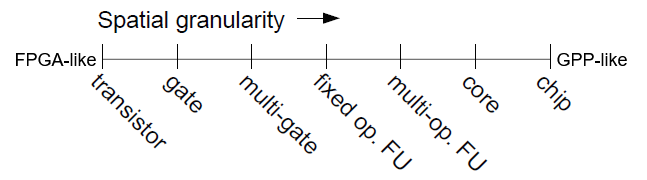
\includegraphics[width=0.49\textwidth]{Figures/Spatial_granularity_edited.png}}
		\subfigure[Temporal granularity levels]{\label{fig:time_granularity} 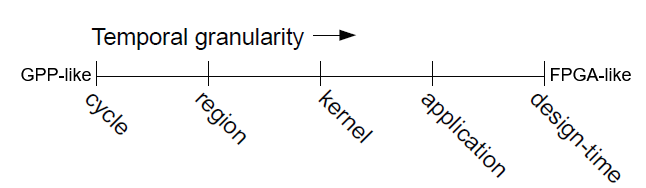
\includegraphics[width=0.49\textwidth]{Figures/Temporal_granularity_edited.png}}	
	\end{subfigmatrix}
	\caption{Spatial and temporal granularity levels, adapted from~\cite{CGRA:Overview2016_wijtvliet}}
	\label{fig:CGRA_granularities}
\end{figure}
CGRAs are integrated in systems mainly as accelerators. The runtime
reconfigurability allows for changes in the datapath, which allows for hardware
reuse in complex applications. At the same time, the FU granularity enables
enough degree of control for applications that do not take advantage of
bit-level manipulation.

With an adequate tool chain for assembly, compilation and place and route, CGRAs
have the potential to facilitate HW acceleration for multiple application types.

Neural networks is one of such applications. All layers in a neural network have
the same elemental operations which are mostly MACs and data
transfers. Therefore, with tailored FUs and correct datapath configuration, a
neural network acceleration environment based on CGRAs seems very attractive.
%One example are neural networks, which are composed of multiple layers. However, all layers have the same elemental operations which are mostly MACs and data transfers. Therefore, with tailored FUs and correct datapath configuration, a neural network acceleration environment based on CGRAs seems very attractive.
\section{Deep Versat}
\label{sec:Deep_Versat}
Deep Versat is a CGRA architecture proposed and implemented
in~\cite{VMario:Deep_Versat}. Deep Versat is composed by Versat Layers disposed
in a ring structure, as presented in Fig.~\ref{fig:DeepVersat_architecture}.

Each Versat Layer is composed of a Configuration Module (CM) and a Data Engine
(DE). This architecture provides a sustainable way to scale the Versat
architecture developed in~\cite{JDLopes:Thesis_Versat}. The scalability comes
from the fact that the inputs from a Versat Layer can select data from the same
Versat Layer or the previous one. With this connection policy, the routing
complexity is independent from the number of deployed Versat Layers.

\begin{figure}[!htb]
	\centering
	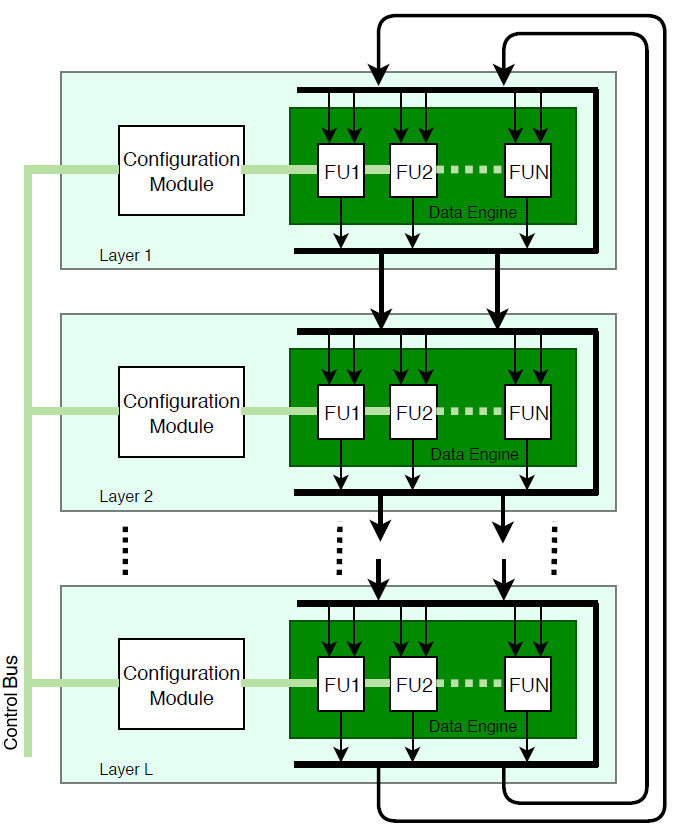
\includegraphics[width=0.5\textwidth]{Figures/deep_versat_arch.png}
	\caption[Caption for figure in TOC.]{Deep Versat architecture, from~\cite{VMario:Deep_Versat}}
	\label{fig:DeepVersat_architecture}
\end{figure}

\subsection{Data Engine}
\label{sec:versat_data_engine}
The Data Engine (DE) at each Versat Layer is where computations take place. The
DE is composed of a set of Functional Units (FUs) in a full-mesh topology. Even
though the number of FUs is variable, the topology presents scalability
problems, so the author recommends configuring the DE so that each FU input can
select one out of a maximum of 20 data sources (10 of then from the previous
Versat Layer). A diagram of a DE is presented in
Fig.~\ref{fig:Versat_data_engine}.

The DE also contains a Configuration Bus to configure each FU with the type
of operation and input selection.

The FUs in a typical DE are Arithmetic and Logic Units (ALUs), multipliers,
barrel shifters and dual-port embedded memories.

All FUs have a single output port with the exception of the dual-port memories,
which have two. The maximum number of FUs is 10, so that the Versat layer does
not produce more than 10 data sources that can be selected by the FUs
themselves.

The dual-port memories have two inputs and outputs and two Address Generation
Units (AGUs) that can generate addresses sequences for the two memory ports. The
AGUs are able to generate addresses for variables in nested double loops. Each
memory port can read from or write to an address generated by its AGU, an
address input to the other port, or can work as a Data Generation Unit (DGU),
outputting the sequence generated by the AGU to the memory port itself.

\begin{figure}[!htb]
	\centering
	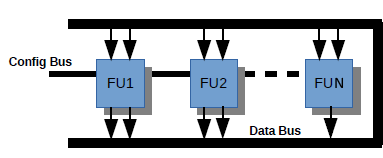
\includegraphics[width=0.5\textwidth]{Figures/versat_data_engine.png}
	\caption[Caption for figure in TOC.]{Versat data engine, adapted from~\cite{VMario:Deep_Versat}}
	\label{fig:Versat_data_engine}
\end{figure}


\subsection{Configuration Module}
\label{sec:versat_config_module}

The Configuration Module (CM) is the module where the DE configurations are
stored and managed. Fig.~\ref{fig:Versat_config_module} presents the structure
of the configuration module. The main components of this module are the
configuration memory, register file and shadow register.

The shadow register holds the configuration currently being executed by the
DE. The existence of this register allows for changes in the register file
without affecting the DE execution.

The configuration register file is composed of configuration spaces that in turn
have multiple configuration fields. One configuration field has the control bits
for a particular feature of a single FU, while a configuration space has the set
of configuration fields for an FU. Each configuration field can vary in bit
width as different the FU features require different numbers of configuration
bits. Configuration fields exploit time locality as the whole DE configuration
chages little over time. Furthermore, by being addressable at the configuration
field level, partial configuration of an FU becomes possible.

The register file takes advantage of time locality, as it is likely that the
same DE configuration is valid for a time span or similar configurations are
used in sequence.

The configuration memory can store 64 full DE configurations, the most used ones
usually, which can be loaded from or uploaded to the register file or external
memory, opening the possibility for more configuration storage in the system.
 

\begin{figure}[!htb]
	\centering
	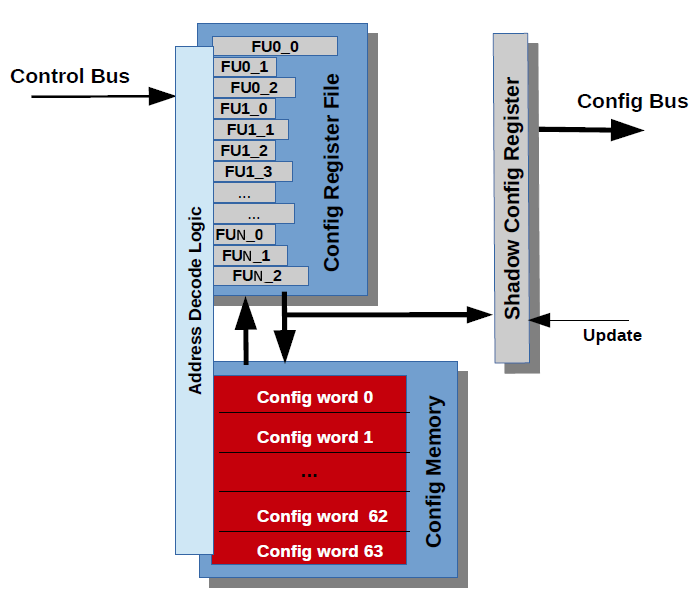
\includegraphics[width=0.5\textwidth]{Figures/versat_config_module_edited.png}
	\caption[Caption for figure in TOC.]{Versat configuration module, adapted from~\cite{JDLopes:Thesis_Versat}}
	\label{fig:Versat_config_module}
\end{figure}


\subsection{Controller and System Integration}
\label{sec:Versat_controller}
The Deep Versat layers are controlled by a soft processor using a RISC-V
architecture. This architecture is programmable with the GNU standard toolchain,
which contains compilers for C and C++.

In~\cite{VMario:Deep_Versat}, Deep Versat is connected to the controller as a
peripheral using the system control bus. It has a data interface connected
to a data bus. Each bus is memory mapped by a distinct memory base address.
There are also dataflow buses that connect two consecutive Versat layers.

The control bus is used to start a Deep Versat run and verify its
completion. Additionally, this bus can access the Versat memory FUs and is also
used to manage the configuration registers and memory.

The data bus connects Deep Versat to data sources and sinks and should be used
for larger and faster data transfers. The author comments on the inefficiency of
driving the data through the RISC-V processor and suggests the implementation of
a DMA engine connecting Deep Versat directly to the external memory instead.
 
Fig.~\ref{fig:DeepVersat_architecture} presents the system architecture, where
there is also a UART peripheral, used mainly for printing debug and verification
messages. Each Versat block represents a Versat layer of Deep Versat.

\begin{figure}[!htb]
	\centering
	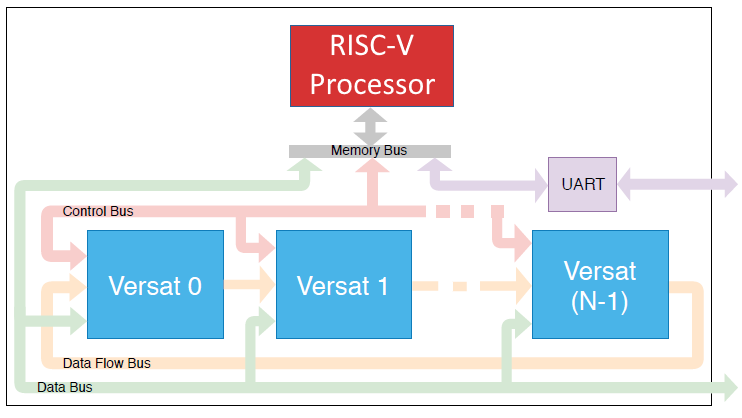
\includegraphics[width=0.6\textwidth]{Figures/deep_versat_system_edited.png}
	\caption[Caption for figure in TOC.]{Deep Versat system, adapted from~\cite{VMario:Deep_Versat}}
	\label{fig:deep_versat_system}
\end{figure}
\subsection{Deep Versat API}
\label{sec:Versat_API}
To facilitate datapath configuration in Deep Versat, an API in C++ was created
where the hardware modules are represented by classes and and their functions and
connections are accessed by the class's methods.

First, the definition of the number of Versat layers, types and number of FUs
and memory sizes is established. Then, the hardware architectural parameters of
Deep Versat are passed into the API via a python script that generates a C++
header file from the Verilog header file containing all the macros used for
pre-silicon configuration.


\section*{Final Remark}
\label{sec:chapter3_conclusion}
CGRAs have the potential to combine the computational capabilities of FPGAs with
the versatility of software, lowering the barrier of entry for model
deployment. For that, the CGRA requires dedicated FUs for the CNN layers that
exploit datapath and model reduction optimizations, while having an adequate
toolchain for software development.
